\documentclass[a4paper]{article}
\usepackage[utf8]{inputenc}
\usepackage{amsfonts}
\usepackage{amsmath}
\usepackage{amsthm}
\usepackage{graphicx}
\usepackage{array}
\usepackage[footnotesize,bf,format=hang]{caption}
\usepackage{mathtools}
\usepackage{booktabs}
\usepackage{subfigure}
\usepackage{textcomp} % For the cent symbol
%\usepackage[font=footnotesize]{subcaption}
\usepackage{varioref}
\captionsetup{justification=justified, singlelinecheck=true}
\usepackage[backend=biber,url=false,doi=true,style=authoryear]{biblatex}
\addbibresource{library.bib}
\usepackage{authblk}
\usepackage{attrib}
\usepackage{enumerate}
%\bibliographystyle{elsarticle-harv}
%\nocite{*}
% % Diagramming
\usepackage{tikz}
\usepackage{float}
\usetikzlibrary{arrows,positioning,decorations}
% %

\title{A global inter-country economic model based on linked input-output models}
\author[*]{Robert G. Levy}
\author[**]{Thomas P. Ol\'{e}ron Evans}
\author[*]{Alan G. Wilson}

\affil[*]{Centre for Advanced Spatial Analysis, UCL Bartlett Faculty of the Built Environment,
90 Tottenham Court Road, London W1T 4TJ, UK}
\affil[**]{Department of Mathematics, University College London, Gower Street, London WC1E 6BT, UK}


\begin{document}
\maketitle

\begin{abstract}
This paper presents a new, flexible and extensible alternative to multi-regional input-output (MRIO) for modelling the global economy.
The limited parameter set of MRIO (technical coefficients only) is extended to include two new set of parameters, import ratios and import propensities.
These new parameter sets assist in the interaction of the new model with other social science models such as those of trade, migration, international security and development aid.
The model uses 40 input-output models from the World Input-Output Database as descriptions of the internal workings of countries' economies, and couples these loosely using trade data for commodities and services from the UN.
The model is constructed using a minimal number of assumptions, seeks to be as parsimonious as possible in terms of the number of parameters, and is based to a great extent on empirical observation.
Some initial analysis is presented (CHANGE THIS).
The new model is shown to be equivalent to an MRIO under an additional assumption, allowing existing techniques for MRIO analysis to also be applied to this model.
\end{abstract}

\section{Introduction}
The objective of this paper is to present a global economic model that can be used as the basis for assessing the impacts of future changes in trade, migration, security and development aid.
The model presented here represents a first `proof of concept' step towards this ambitious goal.
At this stage, the focus is on creating a model of global trade which will form a skeleton onto which additional social science models will be added in future work.
The economies of individual countries are represented as 35-sector input-output models, each of which is linked through trade flows representing imports and exports.
This has recently been made feasible by the publication of the World Input-Output Database (WIOD) \parencite{timmer_world_2012}, a collection of national input-output tables (NIOTs) for 40 countries across 17 years, from 1995 to 2011.
The NIOTs are linked through data from the UN covering trade in both products\footnote{comtrade.un.org/db} and services\footnote{unstats.un.org/unsd/servicetrade/}.

While other models of world trade based on the input-output methodology exist, the model presented here is one of the first to integrate the extremely detailed internal economic data provided by the WIOD with the enormous wealth of trade data from the UN COMTRADE database, resulting in a picture of global trade that includes an unparalleled amount of real economic information.
The use of such extensive data sources and the simplicity and flexibility of the model proposed will allow for the thorough investigation of a broad sweep of economic scenarios in future work.

The remainder of this paper is structured as follows: 
Section \ref{sec:litreview} gives an overview of existing work in this area;
Section \ref{sec:system} gives a description of the present system and outlines how data is used to calibrate the parameters of the model;
The algorithm used to calculate the output of the model is described in section \ref{sec:algorithm} and some preliminary results are given in section \ref{sec:analysis}.
Conclusions and potential directions for future research are presented in section \ref{sec:conclusions}.

\section{Existing Global Economic Models} \label{sec:litreview}
In the mid-1970s, the creator of input-output economics, Wassily Leontief, used the acceptance speech of his Nobel prize in Economics to announce a very ambitious project to model the global economy:

\begin{quotation}
Major efforts are underway to construct a data base for a systematic input-output study not of a single national economy but of the world economy viewed as a system composed of many interrelated parts [...]
Preliminary plans provide for a description of the world economy in terms of twenty-eight groups of countries, with about forty-five productive sectors for each group. \attrib{\cite{leontief_structure_1974}}
\end{quotation}

Twenty years on, Faye Duchin, a former research assistant of Leontief, described how Leontief's efforts in this area had largely been ignored by economists, describing his departures from the standard, neoclassical modelling in terms of price elasticity and elasticity of substitution as being ``too great to ignore'' \parencite{duchin_international_2004}. 
See section \ref{sec:iots} for more on this subject.

In the years since Leontief published his global model, input-output analysis has been largely restricted to regional studies, of which \textcite{akita_interregional_1993}, \textcite{khan_sectoral_1999} and \textcite{luo_power--pull_2013} are examples; and studies related to energy and the environment, such as  \textcite{leontief_environmental_1970}, \textcite{joshi_product_1999}, \textcite{bergh_handbook_2002} and \textcite{hendrickson_environmental_2006}.

However, much more recently, attention has returned to input-output modelling in a global context more generally. \textcite{tukker_global_2013} describe how several multi-regional input-output (MRIO) models have been developed in the very recent literature.
These are, along with the WIOD which is used in the present model, EORA \parencite{lenzen_building_2013}, EXIOPOL \parencite{tukker_exiopol_2013} and the more mature, but proprietorial GTAP \parencite{walmsley_introduction_2012}.

Each of these existing models of the global economy extends the idea of the national input-output table to an international setting: where in an NIOT the magnitude of every bilateral sector--sector flow is recorded for a given country, these projects record the magnitude of every country/sector--country/sector flow.
Thus, for example, the extent to which British agriculture purchases from Belgian manufacturing is recorded in dollar amounts.
This results in a very large matrix which, through inversion in the normal input-output way, can be used to predict the impact of a particular exogenous change in demand.
The authors believe that this is taking the simplicity and elegance of input-output analysis a little far. The idea that each sector buys in fixed proportion from each other sector in each other country turns the above-mentioned ignoring of price- and substitution-elasticities from a convenient simplification in the case of the NIOT to an out-and-out denial of the concept of economic dynamics.

The present model provides a framework in which the power of input-output analysis at the national level can be combined with a more subtle understanding of the dynamics of international trade.
The standard WIOT of $C$ countries and $S$ sectors requires $SC\times SC$ parameters and a major goal of this model is to minimise the number of parameters required to model a global system.
It also provides modellers with a richer set of parameters than the standard technical coefficients of WIOTs which will facilitate the combination of the present model with other models of human systems, such as migration, international security and development aid.

INSERT SELLING SENTENCE

\section{The System Description} \label{sec:system}
The model presented here has $C$ countries, the economies of which are divided into $S$ productive sectors.
Although each sector produces many distinct products, for the sake of simplicity, these products are considered to be perfect substitutes, allowing the terms `sector' and `product' to be used interchangeably throughout this paper.

All product flows are given by value, measured in millions of (current price) US\$.
For the remainder of this paper the terms `quantity' and `value' will therefore also be used interchangeably.
Products produced domestically are labelled with a dagger superscript ($\dagger$) and imported products with an asterisk.

Table \ref{tbl:cvars} shows the quantities taken directly from data published by the WIOD which characterise a country's economy for a particular year. For final demand and investment, the values are summed across the columns mentioned.
\begin{table}
\begin{center}
\begin{tabular}{cp{5cm}l}
\toprule
	            & description                 & source columns \\ \midrule
	$f_s^{(i)}$ & final demand on sector $s$  & 
		\parbox[t]{6cm}{Final consumption expenditure by: \\ households, NPISH \& government} \\
	$n_s^{(i)}$ & investment of sector $s$    & 
		\parbox[t]{6cm}{Gross fixed capital formation, \\
						changes in inventories and valuables}\\
	$e_s^{(i)}$ & exports of sector $s$       & Exports \\
	$z_{s,t}^{\dagger(i)}$ & intermediate demand on 
							sector $s$ by sector $t$ (domestic)& c1--c35 (top section)\\
	$z_{s,t}^{*(i)}$ & intermediate demand on 
							sector $s$ by sector $t$ (imported)& c1--c35 (bottom section)
\\\bottomrule
\end{tabular}
\end{center}
\caption{Quantities from WIOD national input-output tables that define the economy of country $i$}\label{tbl:cvars}
\end{table}
Note that for clarity, no time subscript is added. In future time-series analyses such a subscript would have to be added.

The following rows of the NIOTs are combined into a single `Value Added' flow source (not completely equivalent to ``Value added at basic prices", used in the WIOD), which represents the total value of products produced by each sector after the subtraction of the sum of its intermediate demands on other sectors:
\begin{enumerate}[--]
\itemsep -0.4em 
\item Taxes less subsidies on products
\item CIF/FOB adjustments on exports
\item Direct purchases abroad by residents
\item Purchases on the domestic territory by non-residents
\item Value added at basic prices
\item International transport margins
\end{enumerate}
Although `Value Added' is not used in the current iteration of the model, it provides a loose measure of `profitability' or `efficiency' for each sector that may prove useful in future applications and extensions.

\subsection{Input-Output Tables} \label{sec:iots}
Input-output is, at its heart, an accounting methodology.
The products produced by and imported into a given country in a given year are either: sold as inputs to other sectors (`intermediate supply'); supplied to the `final demand' of consumers and the government; invested; or exported.
The total amount imported and produced must equal the amount used, consumed, invested and exported for each sector.

By simple summation, total production of sector $s$ in country $i$ can be defined as the sum of all intermediate supply, plus supply to final demand, investment and export:
\begin{equation}\label{eqn:x}
x_s^{(i)}=\sum\limits_{t}z_{s,t}^{\dagger(i)} + f_s^{\dagger(i)} + n_s^{\dagger(i)} + e_s^{(i)}
\end{equation}
where $z_{s,t}^{\dagger(i)}$ is the intermediate supply from domestic sector $s$ to sector $t$ in country $i$, $f_s^{\dagger(i)}$ is final demand for domestic sector $s$, $n_s^{\dagger(i)}$ is investment and $e_s^{(i)}$ are exports.
The total import of sector $s$ into country $i$ is the sum of all intermediate supply of imported products, plus demand for and investment of imported products. 
It should be noted that, in this iteration of the model, imported products may not be directly exported, though they may naturally supply intermediate demand of sectors whose output is itself exported.
In other words, \textit{re-exports} are set to zero:
\begin{equation}\label{eqn:m}
m_s^{(i)}=\sum\limits_{t}z_{s,t}^{*(i)} + f_s^{*(i)} + n_s^{*(i)}
\end{equation}

For a particular sector, the phrase `total demand' is used to refer to the sum of final demand, investments and exports, including domestically produced and imported products.

An input-output table, $\boldsymbol{T}^{(i)}$, as described by \textcite{miller_input-output_1985}, is a particular arrangement of these quantities, which provides a clear and compact summary of the structure of a national economy.
Neglecting the $(i)$ superscript for clarity, the input-output table (IOT) is defined as follows:

\begin{equation}\label{eqn:T}
\begin{array}{rc}
\begin{array}{cc} & \mbox{Sector} \end{array} 
& 
\begin{array}{cccc} \hspace*{4mm}1 & \mathellipsis & s & \hspace*{2mm} \mbox{F.D. Inv Exp Tot} \end{array} \vspace*{2mm} \\
\begin{array}{r}
\begin{array}{rc}
\mbox{Domestic} & \left\{ \begin{array}{c}
1 \\
\vdots \\
s
\end{array} \right. \\
\mbox{Imports} & \left\{ \begin{array}{c}
1 \\
\vdots \\
s \\
\end{array} \right.
\end{array} \vspace*{2mm} \\
%\begin{array}{cc} \hspace*{17mm} & \mbox{Value Added} \end{array}
\end{array} &
\left( \begin{array}{ccccccc}
z^{\dag}_{1,1} & \mathellipsis & z^{\dag}_{1,s} & f^\dag_{1} & n^\dag_{1} & e_{1} & x_1 \\
\vdots & \ddots & \vdots & \vdots & \vdots & \vdots & \vdots \\
z^{\dag}_{s,1} & \mathellipsis & z^{\dag}_{s,s} & f^\dag_{s} & n^\dag_{s} & e_{s} & x_{s} \\
z^*_{1,1} & \mathellipsis & z^*_{1,s} & f^*_{1} & n^*_{1} & 0 & i_1 \\
\vdots & \ddots & \vdots & \vdots & \vdots & \vdots & \vdots \\
z^*_{s,1} & \mathellipsis & z^*_{s,s} & f^*_{s} & n^*_{s} & 0 & i_{s} \vspace*{2mm} \\
%v_{1} & \mathellipsis & v_{s} & 0 & 0 & 0 & G
\end{array} \right)
\end{array}
\end{equation}
Table \ref{tbl:cvars} shows a summary of the quantities used in \eqref{eqn:T}.

It will often be convenient to gather those quantities having a single subscript into vectors, and those with two subscripts into matrices. 

We can then characterise a country's economy through the $S$-vectors $\boldsymbol{f}^{(i)}$, $\boldsymbol{n}^{(i)}$ and $\boldsymbol{e}^{(i)}$, and by the $S\times S$ matrices $\boldsymbol{Z}^{\dagger(i)}$ and $\boldsymbol{Z}^{*(i)}$.
In matrix form, $\boldsymbol{T}$ may be written:

\begin{equation}\label{eqn:Tvectorised}
\begin{array}{rcc}
\boldsymbol{T} & = & 
\left(
	\begin{array}{ccccccc}
 & \boldsymbol{Z}^{\dag} & & \boldsymbol{f}^\dag & \boldsymbol{n}^\dag & \boldsymbol{e} & \boldsymbol{x} \\
 & \boldsymbol{Z}^* & & \boldsymbol{f}^* & \boldsymbol{n}^* & \boldsymbol{0} & \boldsymbol{i} \\
	\end{array} 
\right)
\end{array}
\end{equation}

\subsection{A Single Country Model}\label{sec:countries}
In the standard input-output model, each country is described by the input-output table described in section \ref{sec:iots} above.
From the elements of $\boldsymbol{Z}^\dagger$ and $\boldsymbol{Z}^*$, each sector has a complete `recipe' for making its output, in terms of the quantities of each product used as input, both domestic and imported. 

From the elements of $\boldsymbol{T}$ two sets of parameters are now defined which will completely specify the behaviour of a particular country in terms of the internal workings of its economy. For the remainder of this section, the country superscript will be excluded whenever its presence is clear from the context.

\subsubsection*{Technical Coefficients}\label{sec:techcoeffs}
By dividing each intermediate flow by the total output of the sector using the intermediate, we can arrive at a set of \textit{technical coefficients} which define the input of one sector required per unit output of another.
The amount of domestically produced product $r$ required by sector $s$ to produce a single unit of output is thus:
\begin{equation}\label{eq:adagger}
a_{r,s}^\dagger = \frac{z^\dagger_{r,s}}{x_s}
\end{equation}
and
\begin{equation}\label{eq:astar}
a_{r,s}^* = \frac{z^*_{r,s}}{x_s}
\end{equation}
for the equivalent measure for imported $r$. There are therefore $2S \times S$ technical coefficients for each country\footnote{Recall that single year is assumed throughout this treatment.
In time series analyses there will be $2S \times S$ technical coefficients for every country in every year.}.
These technical coefficients allow the intermediate demand to be calculated for any given vector of final, investment and export demands. The total demand (intermediate plus final) for domestically produced sector $s$ is:
$$
x_s = \sum_r{a^\dagger_{s,r}x_r} + f^\dagger_s + n^\dagger_s + e_s 
$$
or, in matrix representation:
\begin{align}
\boldsymbol{x}& = 
\boldsymbol{A^\dagger}\boldsymbol{x}
+ 
\boldsymbol{f^\dagger} + \boldsymbol{n^\dagger} + \boldsymbol{e} 
\label{eqn:xIRIO}
\end{align}
Having calculated total domestic production, we can then calculate the import required to satisfy intermediate and final demands as:
\begin{equation}\label{eqn:mIRIO}
\boldsymbol{m}
=
\boldsymbol{A^*}\boldsymbol{x}
+
\boldsymbol{f^*} + \boldsymbol{n^*} 
\end{equation}
Thus the domestic total production and the imports may be completely determined from the total demand and the technical coefficients.

\subsubsection*{Import Ratios}\label{sec:importratios}

The above description treats domestic and foreign goods as complements of one another, rather than as substitutes.
For example, each aeroplane produced would require some fixed quantity of domestic steel, and a (different) fixed quantity of imported steel.
Inspired by the description given by \textcite{duchin_international_2004} of Leontief's proposed global model, the present model reverses this assumption and treats foreign and domestic products as perfect complements.
Some justification for this assumption is given at the end of this section.

Leontief assumed that engineers in an importing country do not care where a product originated; they will simply know that domestic production does not meet their demand, and instead demand a perfectly-substitutable imported product.
In a similar spirit, when a product in the present model arrives at the shores of an importing country, it enters a theoretical `national warehouse' along with domestically produced products, at which point the two become indistinguishable\footnote{Note that this concept is referred to in \textcite{miller_input-output_1985} as \textit{import similarity}}.
The only thing specified by the model is the fraction of all products used domestically which are supplied by imports. This fraction is assumed to remain fixed per country and per sector, and is called the \textit{import ratio}. It is calculated directly from the country's NIOT as:
\begin{equation}\label{eqn:importratio}
d_s^{(i)} = \frac{m_s^{(i)}}{(x_s^{(i)} - e_s^{(i)} ) + m_s^{(i)}}
\end{equation}
where $x_s^{(i)}$, $e_s^{(i)}$ and $m_s^{(i)}$ are the total production, export and import of sector $s$, calculated via equations \eqref{eqn:x} and \eqref{eqn:m} respectively.
The term $(x_s^{(i)} - e_s^{(i)} )$ represents the products used domestically.
It includes all intermediate demand, including that required to fulfil export requirements, as well as direct flows to final demand and investment, but excludes direct flows to export.
This is because imports may not directly supply export demand as per equation \eqref{eqn:Tvectorised}.

The assumption of fixed import ratios significantly simplifies the model, halving the number of technical coefficients that must be specified for a given country, therefore helping to achieve the goal of model parsimony.
A complete set of inter-sector flows, $\boldsymbol{Z}^{\dagger}$ and $\boldsymbol{Z}^{*}$, relating to both domestically produced and imported products, may be determined from a single set of combined technical coefficients, $\boldsymbol{A}$ (equal to $\boldsymbol{A}^{\dagger} + \boldsymbol{A}^{*}$), along with an $S$-vector, $\boldsymbol{d}$, of import ratios.
Additionally, as mentioned above, this also represents a more plausible assumption of how sectors split their purchasing between domestic and imported.

If the total intermediate flow across both domestic \textit{and} imported products is defined as $\boldsymbol{Z} = \boldsymbol{Z}^{\dagger} + \boldsymbol{Z}^{*}$ then, following equation \eqref{eq:adagger}, the `combined' technical coefficients can be calculated as:
\begin{equation}\label{eqn:a_combined}
a_{r,s} = \frac{z_{r,s}}{x_s}
\end{equation}

Both $\boldsymbol{A}$ and $\boldsymbol{d}$ are calculated directly from data and are fixed parameters of the country model. This model can be used to calculate total demand $\boldsymbol{x}$ from any given set of total demands as per equation \eqref{eqn:xIRIO}:
\begin{equation}
\boldsymbol{x} 
= 
(\boldsymbol{I} - \boldsymbol{\hat{d}})
(
\boldsymbol{Ax} + 
\boldsymbol{f} + \boldsymbol{n}
)
+ \boldsymbol{e}
\label{eqn:xmodel}
\end{equation}
where $\boldsymbol{f} = \boldsymbol{f}^{\dagger} + \boldsymbol{f}^{*}$ and $\boldsymbol{n} = \boldsymbol{n}^{\dagger} + \boldsymbol{n}^{*}$.
 
Then for any given total production, $\boldsymbol{x}$, every individual inter-sector flow can be recovered as follows:
\begin{align}
\boldsymbol{Z}& = \boldsymbol{A}\boldsymbol{\hat{x}}\nonumber\\
\boldsymbol{Z^*}& = \boldsymbol{\hat{d}}\boldsymbol{Z}\\
\boldsymbol{Z^\dagger}& = (\boldsymbol{I} - \boldsymbol{\hat{d}})
	\boldsymbol{Z}\label{eqn:zstar}
\end{align}
Finally, using the definition of the import ratios from equation \eqref{eqn:importratio}, total domestic production $\boldsymbol{x}$ can be used to define imports:
\begin{equation}
\boldsymbol{m} = 
(\boldsymbol{I} - 
\boldsymbol{\hat{d}})^{-1} 
\boldsymbol{\hat{d}}\boldsymbol{x}\label{eqn:mmodel}
\end{equation}
where $\boldsymbol{\hat{d}}$ is an $S \times S$ matrix whose diagonal elements are the import ratios, $d_s$, and $\boldsymbol{I}$ is the appropriately sized identity matrix.

A further benefit for parameter parsimony of the import ratios assumption is that final demand and investment have only $S$ elements to be specified, rather than the $2S$ elements shown in equation \eqref{eqn:T}.
This implies that consumers have no preference between domestic and imported products.
Rather it is up to the sectors to decide how best to meet the single demand for their product.

\subsection{An International Trade Model}\label{sec:trade}
The concept of the NIOT is often expanded to an international context using inter-regional input-output modelling (IRIO). In standard IRIO, each sector in each country is explicit about which countries it gets its imports from. 
This requires each sector to have $S \times C$ technical coefficients, an onerous data requirement and, as already mentioned, a challenge to the credibility of the assumptions required. 

The WIOD present all these technical coefficients in the world input-output tables (WIOTs) which they publish, but the present model instead takes a second assumption from Leontief via \textcite{duchin_international_2004} which he refers to as ``export shares''.

\subsubsection*{Import Propensities}
The assumption is that countries get each of their imported products from their international trading partners in fixed proportions.
Thus, country $j$ will always get the same proportion of its total import demand for product $s$ from country $i$.
We refer to these fixed proportions as \textit{import propensities} as they describe a country's propensity to import a given product from each other country.
The propensity for country $j$ to import product $s$ from country $i$ is given by:
\begin{equation}\label{eqn:importpropensities}
p^{(i,j)}_s = \frac{y^{(i,j)}_s}{\sum_k{y^{(k,j)}_s}}
\end{equation}
where $y^{(i,j)}_s$ is the trade flow of product $s$ from country $i$ to country $j$. The $y_s$ are taken directly from the UN COMTRADE database, with a mapping between the UN's 6-figure product code and the NIOT sector aggregation\footnote{This mapping was provided to us by the team behind the WIOD. This was of invaluable help in creating the present model.}.

Given the import requirements of each country from equation \eqref{eqn:mmodel} and the import propensities from \eqref{eqn:importpropensities}, the export demand on sector $s$ in country $i$ due to demand from country $j$ can be calculated as:
\begin{equation*}
e_s^{(i,j)} = p_s^{(i,j)}m_s^{(j)}
\end{equation*}
and total export demand in country $i$ is therefore:
\begin{equation}\label{eqn:emodel}
e_s^{(i)} = \sum_k{p_s^{(i,k)}m_s^{(k)}}
\end{equation}
\noindent Equations \eqref{eqn:importratio}--\eqref{eqn:emodel} thus describe a system which defines the total productions, $x_s^{(i)}$, of all sectors in all countries; the intermediate input-output flows, $z_{s,t}^{\dagger(i)}$ and $z_{s,t}^{*(i)}$; imports, $m_s^{(i)}$; exports, $e_s^{(i)}$; and all trade flows, $y_s^{(i,j)}$, given a set of technical coefficients, $a_{r,s}^{(i)}$, import ratios, $d_s^{(i)}$, trade propensities, $p_s^{(i,j)}$, and final demands\footnote{In the present version of the model, investments, $n_s^{(i)}$, are set to zero. 
Data on investments is provided by the WIOD but it is not used in this version.}, $f_s^{(i)}$. Folowing a given set of changes to any of the latter four parameters, all of the former six categories of flows can be found.

\subsection{Setting model parameters from data}
As outlined above, the model takes four groups of parameters and produces a complete set of flows within countries (input-output flows) and a complete set of trade flows (imports and exports) between countries. These four groups of parameters are either calculated from the NIOTs provided by the WIOD or from commodity and services trade data provided by the UN.
To recap, the four groups of parameters are:
\begin{enumerate}
\item Final demand, $f_s^{(i)}$: the quantity of a product consumed by the public and the government of a particular country. These are taken directly from the NIOTs using the columns described in table \ref{tbl:cvars}.
\item Technical coefficients, $a_{r,s}^{(i)}$: the quantity of product $r$ required in country $i$ to make a single unit of product $s$. Calculated from the NIOTs using equation \eqref{eqn:a_combined}. 
\item Import ratios, $d_s^{(i)}$: the proportion of country $i$'s total demand for product $s$ which is supplied by imports. Calculated from the NIOTs using equation \eqref{eqn:importratio}.
\item Import propensities, $p_s^{(i,j)}$: the proportion of country $j$'s total of import of product $s$ which comes from country $i$. Calculated from the UN trade data using equation \eqref{eqn:importpropensities}.
\end{enumerate}

\subsection{Modelling the `rest of the world'}\label{sec:RoW}
The UN trade data records flows to and from many countries (as well as many non-country `trade areas') which are not part of the WIOD. If these flows were simply ignored, then countries which trade significantly with these areas would be misrepresented in terms of extent to which they trade with the countries which \textit{are} in the model. To avoid this, the model includes a `rest of the world' entity (RoW) which receives all exports going to countries (`stray' exports) not explicitly modelled, and provides all imports coming from such countries (`stray imports'). The RoW has no technical coefficients and no import ratios.

The RoW is initialised to have a final demand, $f_s$, equal to the total stray exports in each sector across the whole model\footnote{flows from countries not in the model to other countries not in the model are ignored.}. Then, since the RoW has no import ratios, instead of solving equation \eqref{eqn:mmodel} to calculate import demand, it simply sets
\begin{equation}\label{eqn:RoW_imports}
\boldsymbol{m} = \boldsymbol{f}
\end{equation}
thus importing a fixed amount of each sector, defined by the initial level of stray exports in the data.

The RoW also has a particular way of deriving its total production, $\boldsymbol{x}$. It has no technical coefficients, so cannot solve equation \eqref{eqn:xmodel}. Rather, it simply sets
\begin{equation}\label{eqn:RoW_total_production}
\boldsymbol{x} = \boldsymbol{e}
\end{equation}
which allows it to produce `for free' (in the sense that there is no intermediate demand) whatever is required of it from other countries. This also has the effect of decoupling the RoW's import side from its export side.

Other than these aspects, the RoW behaves just like a normal country: it has a set of import propensities relating its imports to each other country, and each other country will have an import propensity relating to trade with the RoW.

\section{Solving the model}\label{sec:algorithm}
To get production requirements from traditional WIOT, it is sufficient to invert the matrix and solve for $\boldsymbol{x}$ directly via Leontief's famous equation:
\begin{equation}
\boldsymbol{x} = (\boldsymbol{I}- \boldsymbol{A})^{-1}\boldsymbol{f}
\end{equation}
The elegance of Leontief's method also had an additional benefit in that it was computationally efficient.
Mathematical methods existed for efficient inversion of matrices which lent the solution extra appeal in an age of hand-wrought numerical solutions.

\subsection{The drawbacks of mathematical elegance}
Behind this elegant and efficient formulation are the assumptions that:
\begin{enumerate}[i]
\itemsep 0em
\item production functions are linear: to produce double the output, double the amount of every input is required,
\item production possibilities are unlimited: an economy will simply produce whatever is demanded of it,
\item markets always clear: all demand is fulfilled immediately.
\end{enumerate}
The undeniable computational convenience of the traditional method of solving IO-models is no longer a sufficient justification for its use, if it is accompanied by assumptions which would not otherwise be made.

The model in its current form relaxes none of the three assumptions given above, but the separation of international trade from individual domestic economies offers the flexibility to do so in future work, simply by making the desired alterations to the country-level model.
Such alterations would be more straightforward to perform and more intuitively comprehensible in this model than in a world input-output table, where changing any individual process would require consideration of the entire system and would likely necessitate a completely new approach to finding solutions.
Recent work on complexity in economics such as \textcite{beinhocker_origin_2006} and \textcite{ramalingam_exploring_2009} supports the thesis that many of the interesting phenomena in macroeconomics happen when systems are out of equilibrium.
With this in mind, a routine is described below for solving the model iteratively, rather than through a single, large matrix inversion.

\subsection{Algorithm for an iterative solution}
\begin{figure}[tb]
\centering %
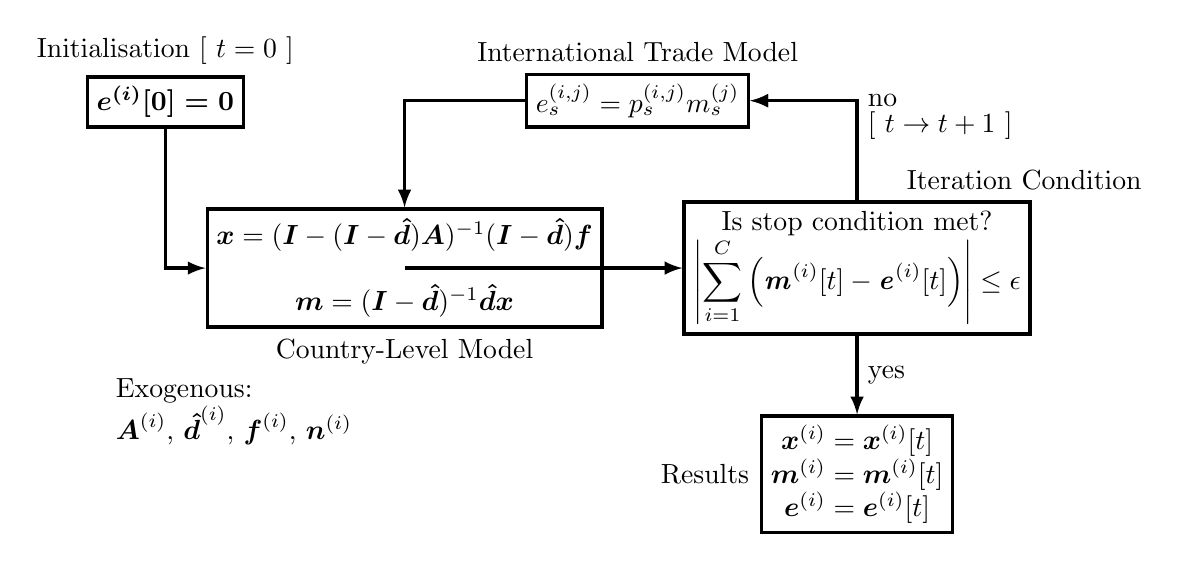
\begin{tikzpicture}[>=latex, very thick]
	\tikzstyle{all nodes}=[shape=rectangle]
	\tikzstyle{box}=[draw]
	% % Nodes
	% init
	\node[box,label=above:{Initialisation [ $t=0$ ]}](init)
	{$\boldsymbol{e^{(i)}[0] = 0}$};
	% country-level model
	\node[box, below right= and -.5cm of init, 
		  align=center, label=below:Country-Level Model]
	(country)
	{
		$
		\boldsymbol{x} = 
		(\boldsymbol{I} - 
		(\boldsymbol{I} - \boldsymbol{\hat{d}})
		\boldsymbol{A})^{-1} 
		(\boldsymbol{I} - \boldsymbol{\hat{d}})\boldsymbol{f}
		$ \\\\
		$
		\boldsymbol{m} = 
		(\boldsymbol{I} - 
		\boldsymbol{\hat{d}})^{-1} 
		\boldsymbol{\hat{d}}\boldsymbol{x}
		$
	};
	% international trade model
	\node[box, above right= and -1cm of country](trade)
	[label=above:International Trade Model]
	{
		$e_s^{(i,j)} = p_s^{(i,j)}m_s^{(j)}$
	};
	% iteration condition
	\node[box, right= of country, align=center](iteration)
	[label=60:Iteration Condition]
	{
		Is stop condition met?
		\\
		$
		\displaystyle \left| \sum^C_{i=1} \left(\textbf{\textit{m}}^{(i)}[t] -
		\textbf{\textit{e}}^{(i)}[t] \right) \right| \leq \epsilon
		$
	};
	% results
	\node[box, below=of iteration, align=center](result)
	[label=left:Results]
	{
		$\boldsymbol{x}^{(i)}=\boldsymbol{x}^{(i)}[t]$ \\
		$\boldsymbol{m}^{(i)}=\boldsymbol{m}^{(i)}[t]$ \\
		$\boldsymbol{e}^{(i)}=\boldsymbol{e}^{(i)}[t]$
	};
	% Exogenous annotation
	\node[below left=0.5cm and -2cm of country, align=left] {
	Exogenous: \\
	$\boldsymbol{A}^{(i)}$,
	$\boldsymbol{\hat{d}}^{(i)}$,
	$\boldsymbol{f}^{(i)}$,
	$\boldsymbol{n}^{(i)}$
	};
	% % Connectors
	\draw [->] (init) |- (country);
	\draw [->] (country) |- (iteration);
	\draw [->] (iteration) |- node[right]{no}(trade);
	\draw [->] (iteration) |- node[below right]{[ $t \rightarrow t+1$ ]}(trade);	
	\draw [->] (trade) -| (country);
	\draw [->] (iteration) -- node[right]{yes}(result);
\end{tikzpicture}
\caption{The model algorithm: total production, imports and exports are calculated for a given set of exogenous parameters. Note that square brackets have been introduced to designate the iteration variable $t$, which tracks the quantities that are iteratively recalculated as the algorithm runs.}\label{fig:algorithm}
\end{figure}

Figure \ref{fig:algorithm} shows a schematic version of the algorithm for calculating imports and exports from the four groups of parameters.
\subsubsection*{Initialisation}
All export demands are set to 0.

\subsubsection*{Country-level model}
Inside each country, total demand is calculated using the export demands (which were initially set to zero), final demands, technical coefficients and import ratios, as per equation \eqref{eqn:xmodel}.
This step maintains the standard input-output matrix inversion.
From total demand, import demand can be calculated via the import ratios as in equation \eqref{eqn:mmodel}.

\subsubsection*{Iteration condition}
At this point a `stop condition' is checked: does the total level of global import demand match total exports in each sector, to within some small value,  $\epsilon > 0$\footnote{More specifically, as shown in Figure \ref{fig:algorithm}, we verify that the length of the vector of differences between the global sum of all imports and the global sum of all exports for each sector does not exceed $\epsilon$. This approach ensures that global export and import totals must balance for all sectors simultaneously.}?
In the first run through the iteration, this stop condition will certainly fail, because exports have just been set to zero.

\subsubsection*{International trade model}
The import demands calculated in the country-level models can be divided up into export demands using the import propensities using to equation \eqref{eqn:emodel}.
These new export demands replace the export demands from the previous iteration (which were all zero the first time round).
With a new set of export demands calculated the algorithm returns to the country-level model.

The iteration continues in this way, moving between the country-level and the international-level models, until the system of imports and exports converges and the stop condition is met \footnote{An analysis of the stability and convergence of the algorithm is the focus of upcoming work by CITE ANTHONY HERE???}.

INSERT SELLING SENTENCE

\section{Analysis}\label{sec:analysis}
The model combining input-output country descriptions and the international trade network allows for the measurement of the total input required to make a single unit of a particular sector's product.
Since the WIOD reports product flows in millions of US dollars (\$M), this will also be the unit of all the following analysis.

\subsection{Simple modelling approaches}
\label{ss_simple_modelling_approaches}

\subsubsection*{Economic significance}
A simple way to measure the significance to the global economy (hereafter `significance') of a sector is to model the reduction of final demand for the products of that sector by one unit, and measure the response of each other sector in each other country in the model. INSERT SELLING SENTENCE

We can formalise the final-demand change in sector $s$ in country $i$ as:

\begin{equation}\label{eqn:reduce_fd_by_one}
f_s^{(i)} \rightarrow f_s^{\prime (i)} \equiv (f_s^{(i)} - 1)
\end{equation}
The simplest way to define `response' is as the change of total output of all sectors, $r$, in all countries, $j$, caused by the reduction:
\begin{equation}
\Delta_{s}^{(i)} x_{r}^{(j)} \equiv (x_{r}^{\prime(j)} - x_r^{(j)})
\end{equation}
where $x_{r}^{\prime(j)}$ is the total output of sector $r$ in country $j$ after the change in equation \eqref{eqn:reduce_fd_by_one} has taken place and the model has been recalculated according to Figure \ref{fig:algorithm}.
$\Delta_{s}^{(i)} x_{r}^{(j)}$ is thus the change in output of sector $r$ in country $j$ induced by the change in final demand for sector $s$ in country $i$.

The total response across all countries and all sectors induced by sector $s$ in country $i$ is:
\begin{equation}
\eta_s^{(i)} \equiv \Delta x_{s}^{(i)} = \sum_j \sum_r \Delta_{s}^{(i)} x_{r}^{(j)}
\end{equation}
and the average response induced by all sectors in country $i$ is:
\begin{equation}
\eta^{(i)} = \frac{\sum_s \eta_s^{(i)}}{S}
\end{equation}
where $S$ is, as before, the number of sectors in country $i$'s economy.

Sectors with a larger value of $\eta_s^{(i)}$ require a larger amount of input to produce each unit of their output. $\eta{(i)}$ can thus be thought of as a country-level significance measure, with larger values implying a economy which, on average, has a greater significance on production in the rest of the world.

Figure \ref{tbl:least_efficient_countries} shows the 10 most significant countries by this measure.
China is the world's most significant economy, a \$1M reduction in final demand leading to an average \$2.36M reduction in total output worldwide.

\begin{figure}
	\centering
	\subfigure[most significant countries]
	{
		\begin{tabular}{lr}
		\toprule
		Country & $\eta^{(i)}$\\
		\midrule
          China &       2.36 \\
 Czech Republic &       1.98 \\
       S. Korea &       1.95 \\
         Russia &       1.94 \\
       Bulgaria &       1.92 \\
          Japan &       1.90 \\
          Italy &       1.90 \\
         Poland &       1.89 \\
        Finland &       1.88 \\
       Portugal &       1.87 \\
		\bottomrule
		\end{tabular}
		\label{tbl:least_efficient_countries}
	}
	\subfigure[China's most significant sectors]
	{
		\begin{tabular}{lr}
		\toprule
		       Sector & $\eta_s^{(\text{China})}$\\
		\midrule
		     Vehicles &       2.47 \\
		         Food &       2.20 \\
		     Plastics &       2.20 \\
		       Metals &       2.17 \\
		    Machinery &       2.17 \\
		         Wood &       2.14 \\
		  Electricals &       2.13 \\
		 Construction &       2.12 \\
		     Textiles &       2.11 \\
		        Paper &       2.10 \\
		\bottomrule
		\end{tabular}
		\label{tbl:chinas_least_efficient_sectors}
	}
	\caption{Response to a \$1M reduction in final demand, in terms of difference induced in the total output, $x$, of other sectors. Only the largest 10 are shown.}
\end{figure}

This is perhaps a surprising result.
How can the US not be the most significant economy in the world?
To investigate further, it is useful to split the significance measure, $\eta^{(i)}$, into foreign and domestic effects, as follows:

\begin{align}
\eta_s^{*(i)} \equiv \Delta x_{s}^{*(i)} & = 
	\sum_{j \neq i} \sum_r \Delta_{s}^{(i)} x_{r}^{(j)} \\
\eta^{*(i)} & = 
	\frac{\sum_s \eta_s^{*(i)}}{s}
\end{align}
and
\begin{align}
\eta_s^{\dagger(i)} \equiv \Delta x_{s}^{\dagger(i)} & = 
	\sum_r \Delta x_{sr}^{(ii)} \\
\eta^{\dagger(i)} & = 
	\frac{\sum_s \eta_s^{\dagger(i)}}{s}
\end{align}
such that
\begin{equation}
\eta^{(i)} = \eta^{*(i)} + \eta^{\dagger(i)}
\end{equation}
Figure \ref{fig:countries_domestic_vs_foreign} shows how the average response across all sectors divides between domestic response, $\eta_s^{\dagger}$, and foreign response, $\eta_s^{*}$, for each country. 
An OLS regression line has been added to the plot.
All the countries lying close to the line have a similar total significance, $\eta^{(i)}$.
The region below the line is the region of less-than-average significance and that above the line is the region of greater-than-average significance.
China is immediately visible as an outlier.
Its economy is around one-third more significant ($\eta = 2.36$) than that of Brazil ($\eta = 1.75$) or India ($\eta = 1.74$), but almost all of this extra significance relates to its impact on its own domestic sectors.
Thus China's significance to the world economy shows itself largely in China itself. China is significant to the extent that it uses disproportionately large amounts of its own productive output in its production technology.
This may perhaps be evidence of the much-vaunted end of low labour costs in China  \parencite{li_end_2012, the_economist_end_2012} although further research would be needed to verify this.

\begin{figure}
\centering
\includegraphics[width=\textwidth]{"images/country response domestic vs foreign - tweaked".pdf}
\caption{The total response of the global economy to a reduction in final demand, averaged across every sector in a country. 
`Response' is defined as the total production lost across all sectors.
Here, response has been divided into domestic, where the response is measured only in the country whose final demand has been reduced, and foreign, where the response is measured in all other countries only.
The solid line shows the result of an OLS regression, with the grey shaded area being the 5\% confidence interval.}
\label{fig:countries_domestic_vs_foreign}
\end{figure}

\subsubsection*{Economic self-reliance}
Countries further to the left of Figure \ref{fig:countries_domestic_vs_foreign}, such as Brazil, India, Japan, Russia, Turkey and the USA, are more self-reliant than those on the right, such as Luxembourg, Belgium, the Netherlands and Denmark.
This self-reliance can be made precise by measuring the ratio of domestic response to foreign response:
\begin{equation}
\phi^{(i)} = \frac{\eta^{*(i)}}{\eta^{\dagger(i)}}
\end{equation}
Figure \ref{fig:phi-vs-pop} shows the relationship between $\phi^{(i)}$ and population in 2010 (World Development Indicators, The World Bank).

The positive slope of the regression line (significant at 0.1\%) indicates that larger countries are generally more self-reliant.
Brazil and Australia are both more self-reliant than their population would suggest.
Belgium and the Netherlands are less self-reliant in the same sense.
Further research might be put into which sectors cause the largest share of these atypical self-reliance measures, particularly that of Brazil as that country is the largest outlier by a wide margin.

\begin{figure}[tb]
\centering
\includegraphics[width=\textwidth]{"images/phi vs population - tweaked".pdf}
\caption{}
\label{fig:phi-vs-pop}
\end{figure}

\subsection{A unified network approach}
The flow of products between countries can be viewed as a weighted, directed network, where countries are nodes, and the weights of each edge represents the magnitude of the flow between them \parencite{nystuen_graph_1961,serrano_topology_2003,bhattacharya_international_2008,baskaran_heckscher-ohlin_2011}.
Similarly with the sector-sector flows which constitute an input-output model \parencite{blochl_vertex_2011,fedriani_simplifying_2012}.
Network science has developed useful ways to analyse the sort of weighted, directed networks which the constitute the present model, but a single network representation is required which combines the international and the sub-national networks.

Recall from section \ref{sec:importratios} above, that products arriving at the shores of an importing country are put into a warehouse along with domestically produced products, at which point the two become indistinguishable.
If an additional assumption is made that domestic sectors take from this warehouse by means of a random sample, then the fraction of products in each sample from abroad will be identical, as will the fraction of imported products from each exporter.
These fractions will be set by the import ratios and import propensities respectively.

This additional assumption allows us to specify a complete system of intermediate (input-output) flows, $y_{rs}^{(i,j)}$, from sector $r$ in country $i$ to sector $s$ in country $j$, thereby effectively reconstructing the WIOT which was diverted from in section \ref{sec:algorithm}:

\begin{equation}\label{eqn:y_rsij}
y_{rs}^{(i,j)} = p_{r}^{(i,j)} d_{r}^{(j)} a_{rs}^{(j)} x_{s}^{(j)}
\end{equation}
Equation \eqref{eqn:y_rsij} can be understood as follows:
sector $s$ in country $j$ requires an amount $a_{rs}^{(j)} x_{s}^{(j)}$ of sector $r$'s product to produce its total output;
a fraction $d_{r}^{(j)}$ of this will be supplied by imports;
a fraction $p_{r}^{(i,j)}$ of these imports will come from country $i$. Note that since countries do not import their own exports, $p_s^{(i,i)}=0,\ \forall i$, and the expression holds trivially for $i=j$.

The fractions of each type of demand for $s$ in country $j$ which was exported by country $i$ are given by similar expressions:

\begin{subequations}
\begin{equation}\label{eqn:f_sij}
f_{s}^{(i,j)} = p_{s}^{(i,j)} d_{s}^{(j)} f_{s}^{(j)}
\end{equation}
\begin{equation}\label{eqn:e_sij}
e_{s}^{(i,j)} = p_{s}^{(i,j)} d_{s}^{(j)} e_{s}^{(j)}
\end{equation}
\begin{equation}\label{eqn:n_sij}
n_{s}^{(i,j)} = p_{s}^{(i,j)} d_{s}^{(j)} n_{s}^{(j)}
\end{equation}
\end{subequations}
where, as previously, $f$ is final demand, $e$ is export demand and $n$ are investments.

Along with the sector-to-sector flows given by equation \eqref{eqn:zstar}, this allows for the representation of all the flows in the present model as a single network, to which standard network analysis techniques can then be applied.

\begin{figure}[tb]
\centering
\includegraphics[width=\textwidth]{"images/Chinese Vehicles Top 10 Countries".png}
\caption{A network representation of the seven most-affected countries following a reduction in final demand for the Chinese vehicles sector. Node size is proportional to eigenvector centrality, and edge width is proportional to the change in flow.}\label{fig:chnvehtop6}
\end{figure}

This reformulation demonstrates the connection between the model described in this paper and the established world input-output table approach, allowing us to visualise the individual country-sector to country-sector flows (or changes in such flows) for any model scenario, such as that calculated in section \ref{ss_simple_modelling_approaches} in response to a reduction of demand in China for the Vehicles sector by \$1M.

The change to every such flow (both $y_{rs}^{(i,j)}$ and $z_{rs}^{(i)}$ type flows) in the eight most-affected countries is recorded and visualised in figure \ref{fig:chnvehtop6}.
Node size is proportional to eigenvector centrality and the edge weight is proportional to the change induced in the particular flow be the reduction in final demand.
This diagram reveals the patterns and shapes of the various economies which would be hard to pick out in the raw flow matrix.


\section{Conclusions}\label{sec:conclusions}
This paper has presented a new model of global trade which separates the modelling approach to the internal workings of an economy and the global trade network. 
It is solved iteratively, thereby avoiding the limitations and assumptions of the traditional world input-output table approach which are less necessary in this age of very fast computing.
The model is extensible to allow for the addition of non-linear production functions, limited production capacities and non-clearing markets.
It also offers a richer set of parameters, with the addition of import ratios and import propensities, which will help integrate it with other social science models, such as those which model how countries choose to trade with one another.

A new measure (SELL MORE - A \textbf{WONDROUS} NEW MEASURE)  of the economic significance of a sector was introduced, and China was found to be a significant outlier in its economic significance in domestic terms.
A measure of economic self-reliance was introduced which was found to vary inversely with population.

Finally, a route from the model presented back to a traditional world input-output table approach, allowing access to analysis from the network science literature, of which a very simple example was presented.

Further work should be done on combining this model with other social science models, particularly those of migration, trade, international security and development aid, and also with the relaxing of the traditional input-output assumptions mentioned above, perhaps starting with production limits.

INSERT SELLING PARAGRAPH

\printbibliography

\end{document} 
